\documentclass[preprint,12pt]{elsarticle}
%DIF LATEXDIFF DIFFERENCE FILE
%DIF DEL /tmp/orig.tex             Sat Sep 26 20:29:50 2026
%DIF ADD pgsg_2_template-num.tex   Sun Sep 27 00:33:01 2026

\usepackage{amsmath,amssymb}
\usepackage{graphicx}
\usepackage{booktabs}
\usepackage{longtable}
\usepackage{hyperref}
\usepackage{lineno}
\modulolinenumbers[5]

\journal{Chemometrics and Intelligent Laboratory Systems}
%DIF PREAMBLE EXTENSION ADDED BY LATEXDIFF
%DIF CFONT PREAMBLE %DIF PREAMBLE
\RequirePackage{color}\definecolor{RED}{rgb}{1,0,0}\definecolor{BLUE}{rgb}{0,0,1} %DIF PREAMBLE
\DeclareOldFontCommand{\sf}{\normalfont\sffamily}{\mathsf} %DIF PREAMBLE
\providecommand{\DIFaddtex}[1]{{\protect\color{blue} \sf #1}} %DIF PREAMBLE
\providecommand{\DIFdeltex}[1]{{\protect\color{red} \scriptsize #1}} %DIF PREAMBLE
%DIF SAFE PREAMBLE %DIF PREAMBLE
\providecommand{\DIFaddbegin}{} %DIF PREAMBLE
\providecommand{\DIFaddend}{} %DIF PREAMBLE
\providecommand{\DIFdelbegin}{} %DIF PREAMBLE
\providecommand{\DIFdelend}{} %DIF PREAMBLE
\providecommand{\DIFmodbegin}{} %DIF PREAMBLE
\providecommand{\DIFmodend}{} %DIF PREAMBLE
%DIF FLOATSAFE PREAMBLE %DIF PREAMBLE
\providecommand{\DIFaddFL}[1]{\DIFadd{#1}} %DIF PREAMBLE
\providecommand{\DIFdelFL}[1]{\DIFdel{#1}} %DIF PREAMBLE
\providecommand{\DIFaddbeginFL}{} %DIF PREAMBLE
\providecommand{\DIFaddendFL}{} %DIF PREAMBLE
\providecommand{\DIFdelbeginFL}{} %DIF PREAMBLE
\providecommand{\DIFdelendFL}{} %DIF PREAMBLE
%DIF HYPERREF PREAMBLE %DIF PREAMBLE
\providecommand{\DIFadd}[1]{\texorpdfstring{\DIFaddtex{#1}}{#1}} %DIF PREAMBLE
\providecommand{\DIFdel}[1]{\texorpdfstring{\DIFdeltex{#1}}{}} %DIF PREAMBLE
\providecommand{\DIFscaledelfig}{0.5}
%DIF HIGHLIGHTGRAPHICS PREAMBLE %DIF PREAMBLE
\RequirePackage{settobox} %DIF PREAMBLE
\RequirePackage{letltxmacro} %DIF PREAMBLE
\newsavebox{\DIFdelgraphicsbox} %DIF PREAMBLE
\newlength{\DIFdelgraphicswidth} %DIF PREAMBLE
\newlength{\DIFdelgraphicsheight} %DIF PREAMBLE
% store original definition of \includegraphics %DIF PREAMBLE
\LetLtxMacro{\DIFOincludegraphics}{\includegraphics} %DIF PREAMBLE
\providecommand{\DIFaddincludegraphics}[2][]{{\color{blue}\fbox{\DIFOincludegraphics[#1]{#2}}}} %DIF PREAMBLE
\providecommand{\DIFdelincludegraphics}[2][]{% %DIF PREAMBLE
\sbox{\DIFdelgraphicsbox}{\DIFOincludegraphics[#1]{#2}}% %DIF PREAMBLE
\settoboxwidth{\DIFdelgraphicswidth}{\DIFdelgraphicsbox} %DIF PREAMBLE
\settoboxtotalheight{\DIFdelgraphicsheight}{\DIFdelgraphicsbox} %DIF PREAMBLE
\scalebox{\DIFscaledelfig}{% %DIF PREAMBLE
\parbox[b]{\DIFdelgraphicswidth}{\usebox{\DIFdelgraphicsbox}\\[-\baselineskip] \rule{\DIFdelgraphicswidth}{0em}}\llap{\resizebox{\DIFdelgraphicswidth}{\DIFdelgraphicsheight}{% %DIF PREAMBLE
\setlength{\unitlength}{\DIFdelgraphicswidth}% %DIF PREAMBLE
\begin{picture}(1,1)% %DIF PREAMBLE
\thicklines\linethickness{2pt} %DIF PREAMBLE
{\color[rgb]{1,0,0}\put(0,0){\framebox(1,1){}}}% %DIF PREAMBLE
{\color[rgb]{1,0,0}\put(0,0){\line( 1,1){1}}}% %DIF PREAMBLE
{\color[rgb]{1,0,0}\put(0,1){\line(1,-1){1}}}% %DIF PREAMBLE
\end{picture}% %DIF PREAMBLE
}\hspace*{3pt}}} %DIF PREAMBLE
} %DIF PREAMBLE
\LetLtxMacro{\DIFOaddbegin}{\DIFaddbegin} %DIF PREAMBLE
\LetLtxMacro{\DIFOaddend}{\DIFaddend} %DIF PREAMBLE
\LetLtxMacro{\DIFOdelbegin}{\DIFdelbegin} %DIF PREAMBLE
\LetLtxMacro{\DIFOdelend}{\DIFdelend} %DIF PREAMBLE
\DeclareRobustCommand{\DIFaddbegin}{\DIFOaddbegin \let\includegraphics\DIFaddincludegraphics} %DIF PREAMBLE
\DeclareRobustCommand{\DIFaddend}{\DIFOaddend \let\includegraphics\DIFOincludegraphics} %DIF PREAMBLE
\DeclareRobustCommand{\DIFdelbegin}{\DIFOdelbegin \let\includegraphics\DIFdelincludegraphics} %DIF PREAMBLE
\DeclareRobustCommand{\DIFdelend}{\DIFOaddend \let\includegraphics\DIFOincludegraphics} %DIF PREAMBLE
\LetLtxMacro{\DIFOaddbeginFL}{\DIFaddbeginFL} %DIF PREAMBLE
\LetLtxMacro{\DIFOaddendFL}{\DIFaddendFL} %DIF PREAMBLE
\LetLtxMacro{\DIFOdelbeginFL}{\DIFdelbeginFL} %DIF PREAMBLE
\LetLtxMacro{\DIFOdelendFL}{\DIFdelendFL} %DIF PREAMBLE
\DeclareRobustCommand{\DIFaddbeginFL}{\DIFOaddbeginFL \let\includegraphics\DIFaddincludegraphics} %DIF PREAMBLE
\DeclareRobustCommand{\DIFaddendFL}{\DIFOaddendFL \let\includegraphics\DIFOincludegraphics} %DIF PREAMBLE
\DeclareRobustCommand{\DIFdelbeginFL}{\DIFOdelbeginFL \let\includegraphics\DIFdelincludegraphics} %DIF PREAMBLE
\DeclareRobustCommand{\DIFdelendFL}{\DIFOaddendFL \let\includegraphics\DIFOincludegraphics} %DIF PREAMBLE
%DIF COLORLISTINGS PREAMBLE %DIF PREAMBLE
\RequirePackage{listings} %DIF PREAMBLE
\RequirePackage{color} %DIF PREAMBLE
\lstdefinelanguage{DIFcode}{ %DIF PREAMBLE
%DIF DIFCODE_CFONT %DIF PREAMBLE
  moredelim=[il][\color{red}\scriptsize]{\%DIF\ <\ }, %DIF PREAMBLE
  moredelim=[il][\color{blue}\sffamily]{\%DIF\ >\ } %DIF PREAMBLE
} %DIF PREAMBLE
\lstdefinestyle{DIFverbatimstyle}{ %DIF PREAMBLE
	language=DIFcode, %DIF PREAMBLE
	basicstyle=\ttfamily, %DIF PREAMBLE
	columns=fullflexible, %DIF PREAMBLE
	keepspaces=true %DIF PREAMBLE
} %DIF PREAMBLE
\lstnewenvironment{DIFverbatim}[1][]{\lstset{style=DIFverbatimstyle}}{} %DIF PREAMBLE
\lstnewenvironment{DIFverbatim*}[1][]{\lstset{style=DIFverbatimstyle,showspaces=true}}{} %DIF PREAMBLE
\lstset{extendedchars=\true,inputencoding=utf8}

%DIF END PREAMBLE EXTENSION ADDED BY LATEXDIFF

\begin{document}

\begin{frontmatter}

\title{\DIFaddbegin \DIFadd{Gate Topology and Reproducibility of }\DIFaddend Prior-Guided Spectral Gating \DIFdelbegin \DIFdel{Generalizes }\DIFdelend Across \DIFdelbegin \DIFdel{Spectroscopic Modalities: Evidence from }\DIFdelend Near-Infrared and Raman Spectroscopy}

% *** PLACEHOLDER: author list, order, and affiliations have not been
% confirmed by the corresponding author. Verify before submission. ***
%\author{Guilherme Coelho$^a$, Clarimar José Coelho$^c$} %% Author name

\iffalse
%% Author affiliation
\author{Guilherme Coelho$^a$,  Clarimar José Coelho$^b$} %% Author name
\affiliation{organization={$^a$State University of Campinas}, 
            {Cidade Universitária Zeferino Vaz - Barão Geraldo}, 
            city={Campinas},
            postcode={13083--970}, 
            state={São Paulo},
            country={Brazil}}
\affiliation{organization={$^c$Postgraduate Program in Industrial Engineering and Artificial Intelligence} Pontificia Universidade Catolica de Goias,
            addressline={Primeira Avenida, s/n - Quadra 88 - Setor Leste Universitário}, 
            city={Goiânia},
            postcode={74605--010}, 
            state={Goiás},
            country={Brazil} }
\fi            
\author[unicamp]{Guilherme Coelho}
\author[puc]{Clarimar José Coelho\corref{cor1}}
\ead{clarimar@pucgoias.edu.br}
\cortext[cor1]{Corresponding author.}
\address[unicamp]{State University of Campinas, 
            Cidade Universitária Zeferino Vaz - Barão Geraldo, 
            Campinas,
            13083--970, 
            São Paulo,
            Brazil}
\address[puc]{Postgraduate Program in Industrial Engineering and Artificial Intelligence Pontificia Universidade Catolica de Goias, Primeira Avenida, s/n - Quadra 88 - Setor Leste Universitário, 
            Goiânia, 74605--010, Goiás, Brazil} 


\begin{abstract}
Prior-Guided Spectral Gating (PGSG) is a \DIFdelbegin \DIFdel{chemometrically-informed }\DIFdelend spectral attention mechanism \DIFdelbegin \DIFdel{, previously validated }\DIFdelend \DIFaddbegin \DIFadd{in which a learnable per-variable sigmoid gate, initialized from a literature-derived prior, weights the spectrum before a shallow multilayer perceptron. It has so far been studied }\DIFaddend only on near-infrared (NIR) spectroscopy\DIFdelbegin \DIFdel{, where it outperforms partial least squares (PLS) at scale ($n\approx1{,}448$, $R^{2}=0.806$ versus $0.568$). Whether the mechanism generalizes to modalities with markedly different spectral structure, such as Raman, has not been tested. We evaluate }\DIFdelend \DIFaddbegin \DIFadd{. We apply }\DIFaddend the unmodified architecture \DIFdelbegin \DIFdel{--- an independent sigmoid gate per variable feeding a shallow multilayer perceptron, trained end-to-end --- on }\DIFdelend \DIFaddbegin \DIFadd{to }\DIFaddend public NIR ($n=1{,}448$, \DIFdelbegin \DIFdel{dry-matter content}\DIFdelend \DIFaddbegin \DIFadd{mango dry matter}\DIFaddend ) and Raman ($n=6{,}472$, glucose\DIFdelbegin \DIFdel{concentration) benchmarks , and formalize three descriptors of learned-gate topology (entropy, smoothness, sparsity) to characterize cross-modality structural differences. The model outperforms PLS in both modalities ($\Delta R^{2}_{\mathrm{PLS}}=+0.244$ NIR , $+0.025$ Raman }\DIFdelend ) \DIFdelbegin \DIFdel{; }\DIFdelend \DIFaddbegin \DIFadd{benchmarks and ask three questions: whether the model outperforms partial least squares (PLS), how the learned gate topology differs between modalities, and what a literature-informed prior contributes. Against PLS with the number of latent variables selected by cross-validation (one-standard-error rule), and with train/test splits that keep replicate spectra of the same sample together, the model does not outperform PLS in NIR (paired $\Delta R^{2}=-0.108\pm0.031$ over ten splits, lower in all ten) but does in Raman ($\Delta R^{2}=+0.036\pm0.007$, higher in all ten). The NIR advantage reported with a fixed, under-parameterized PLS baseline ($+0.23$) disappears once the baseline is calibrated. The learned gates nevertheless differ between modalities in a physically consistent way: }\DIFaddend Raman gates are \DIFdelbegin \DIFdel{more sparse }\DIFdelend \DIFaddbegin \DIFadd{sparser }\DIFaddend than NIR gates, and NIR gates are smoother \DIFdelbegin \DIFdel{than Raman gates }\DIFdelend once smoothness is normalized by physical band density, a correction we show to be necessary\DIFdelbegin \DIFdel{and that reverses the naive raw-index comparison}\DIFdelend . A literature-informed prior does not \DIFdelbegin \DIFdel{improve accuracy over an uninformed initialization }\DIFdelend \DIFaddbegin \DIFadd{change accuracy }\DIFaddend but substantially increases gate reproducibility across training seeds (pairwise Jaccard similarity $0.90$--$0.94$ versus \DIFdelbegin \DIFdel{$0.58$}\DIFdelend \DIFaddbegin \DIFadd{$0.60$}\DIFaddend --$0.65$). A \DIFdelbegin \DIFdel{finer, }\DIFdelend band-level test \DIFdelbegin \DIFdel{cor}\DIFdelend relating local gate structure \DIFdelbegin \DIFdel{with literature-reported vibrational linewidths did not yield a robust correlation. These results indicate that PGSG generalizes across spectroscopic modalities without architectural modification, that the magnitude of its advantage scales with how diluted the analyte signal already is in a given modality, and that the principal value of a physically motivated prioris interpretive stabilityrather than predictive gain. }\DIFdelend \DIFaddbegin \DIFadd{to vibrational linewidths was negative. Since an uninformed initialization reaches the same accuracy, the predictive gain in Raman belongs to the non-linear regressor rather than to the prior, whose value lies in interpretive stability. Predictive claims for neural spectral models require a baseline whose complexity is selected from the data and a validation design that respects replicate structure.
}\DIFaddend \end{abstract}

\begin{keyword}
spectral gating \sep interpretable deep learning \sep Raman spectroscopy \sep near-infrared spectroscopy \sep chemometrics \sep cross-modality generalization
\end{keyword}

\end{frontmatter}

\linenumbers

\section{Introduction}
\label{sec:intro}

Prior-Guided Spectral Gating (PGSG) is a chemometrically-informed attention mechanism for spectroscopic regression, in which a learnable gate $g\in(0,1)^{p}$ over $p$ spectral variables is initialized from a literature-derived prior $s$, rather than from the training data, and multiplies the input spectrum before a downstream regressor. The mechanism was originally established on near-infrared (NIR) spectroscopy at small sample sizes \cite{coelho_pgsg0}. \DIFdelbegin \DIFdel{A subsequent study revised the architecture --- replacing an earlier }\DIFdelend \DIFaddbegin \DIFadd{The present study uses a revised formulation of the architecture, developed within the same research program and fully specified in Section~\ref{sec:architecture}: the original }\DIFaddend formulation, in which a softmax gate weighted a partial-least-squares (PLS) regressor optimized by finite-difference gradients, \DIFdelbegin \DIFdel{with }\DIFdelend \DIFaddbegin \DIFadd{is replaced by }\DIFaddend an independent sigmoid gate per variable feeding a lightweight multilayer perceptron (MLP) trained end-to-end via automatic differentiation\DIFdelbegin \DIFdel{--- and showed that the revised model}\DIFdelend , hereafter \texttt{PGSGv2Model}\DIFdelbegin \DIFdel{, retains a predictive advantage over PLS at substantially larger sample sizes ($n\approx1{,}448$, mango dry-matter content via NIR, $R^{2}=0.806$ versus $0.568$) \cite{coelho_pgsg1,anderson2020}}\DIFdelend .

\DIFdelbegin \DIFdel{Both studies validated PGSG }\DIFdelend \DIFaddbegin \DIFadd{PGSG has so far been evaluated }\DIFaddend exclusively on NIR, leaving open a basic question about the generality of the mechanism: does prior-guided gating help because of a property specific to NIR spectra, or does it reflect a principle applicable across spectroscopic modalities with different physical structure? NIR spectra are dominated by broad, overlapping overtone and combination bands, in which analyte-relevant signal is typically diluted across many correlated wavelengths \cite{workman2012nir}. Raman spectra, by contrast, exhibit narrow, well-resolved vibrational peaks superimposed on a \DIFdelbegin \DIFdel{comparatively flat baseline }\DIFdelend \DIFaddbegin \DIFadd{broad fluorescence background, which becomes approximately flat only after baseline correction }\DIFaddend \cite{smith2019raman}. If the value of prior-guided gating in NIR derives from down-weighting broad, uninformative regions in favor of a chemically relevant subset, the mechanism might contribute comparatively little in a modality where informative peaks are already narrow and readily isolated by the regressor.

We test this directly by applying the unmodified \texttt{PGSGv2Model} architecture to a Raman regression task\DIFaddbegin \DIFadd{, by comparing it against a PLS baseline whose number of latent variables is selected by cross-validation, }\DIFaddend and by formalizing quantitative descriptors of learned-gate topology --- entropy, smoothness, and sparsity --- to characterize \emph{how}, not merely \emph{whether}, gate structure differs between the two modalities. We evaluate five falsifiable hypotheses (Section~\ref{sec:hypotheses}) end to end on public NIR and Raman benchmarks and, in the interest of transparency, document \DIFaddbegin \DIFadd{two corrections made during this study: }\DIFaddend a model-identity error \DIFdelbegin \DIFdel{made during executionof this study that initially produced results opposite to those reported here for the central hypothesis }\DIFdelend \DIFaddbegin \DIFadd{during execution, and a fixed-complexity PLS baseline in the submitted version whose calibration reversed the conclusion for H1 }\DIFaddend (Section~\ref{sec:model-identity}).

\section{Scope}
\label{sec:scope}

An early planning stage of this work considered simultaneous generalization to four modalities: NIR, Raman, mid-infrared (MIR), and mass spectrometry (MS). This scope was narrowed to two modalities for two reasons. First, validating across four modalities within a single study \DIFdelbegin \DIFdel{risks the inverse of a problem already identified and corrected in prior work \cite{coelho_pgsg1}: }\DIFdelend \DIFaddbegin \DIFadd{would create }\DIFaddend an empirical scope exceeding what can be executed and tested with rigor. Second, the physical argument motivating spectral gating --- correlation between adjacent positions along a continuous spectral axis --- does not hold for MS, whose signals are discrete mass-to-charge values without an analogous local neighborhood structure; including MS without adapting the gating operator itself would constitute a weak extension. MIR and MS therefore remain outside the empirical scope of this study.

\section{Hypotheses}
\label{sec:hypotheses}

\begin{description}
\item[H1 (generalization without architectural change).] \texttt{PGSGv2Model}, applied to Raman data without architectural modification (only reconfiguration of the initialization prior), outperforms PLS, reproducing the NIR result qualitatively ($\Delta R^{2}_{\mathrm{PLS}}>0$).
\item[H2 (differential sparsity).] The gate learned on Raman data is significantly more sparse (Hoyer index) than the gate learned on NIR data, reflecting the narrow-peak structure of Raman scattering relative to the broad, overlapping overtone and combination bands of NIR.
\item[H3 (differential smoothness).] The gate learned on NIR data is significantly smoother (normalized total variation) than on Raman.
\item[H4 (value of a physically motivated prior).] Initializing the gate from literature-derived vibrational assignments, rather than from an uninformed initialization, yields predictive performance that is equal to or better, and gate stability across training seeds that is greater, in both modalities.
\item[H5 (structure--physics correlation).] The entropy and smoothness of the learned gate correlate with the known spectral bandwidth of the vibrational transitions relevant to the target analyte, within a given modality.
\end{description}

\section{Materials and Methods}
\label{sec:methods}

\subsection{Datasets}
\label{sec:datasets}

The NIR branch reuses the Mango DMC v3 dataset (dry-matter content, \%; $n=1{,}448$ \DIFdelbegin \DIFdel{in }\DIFdelend \DIFaddbegin \DIFadd{spectra from }\DIFaddend Season~4\DIFdelbegin \DIFdel{, the invariant test season used throughout) \cite{anderson2020}and the associated }\DIFdelend \DIFaddbegin \DIFadd{) \cite{anderson2020}, with a }\DIFaddend literature-derived prior \DIFdelbegin \DIFdel{from the prior study \cite{coelho_pgsg1,saranwong2004}}\DIFdelend \DIFaddbegin \DIFadd{\cite{saranwong2004} (Section~\ref{sec:priors})}\DIFaddend . The Raman branch uses \texttt{bioprocess\_substrates} \cite{lange2026}, a bioprocess-monitoring benchmark accessed through the RamanBench collection \cite{koddenbrock2026}, with glucose concentration as the regression target. Of 6,960 spectra in the source dataset, 6,472 carry a valid glucose label and were retained ($p=1{,}870$ Raman-shift variables spanning 390.6--3384.7~cm$^{-1}$). \DIFaddbegin \DIFadd{Both datasets contain replicate spectra of the same physical sample: the 1,448 NIR spectra come from 725 fruits (723 fruits measured twice, with identical metadata and dry-matter value), and the 6,472 Raman spectra from 3,191 distinct mixtures (identical concentration vectors; mostly duplicate acquisitions). }\DIFaddend Table~\ref{tab:datasets} summarizes both branches.

This dataset was selected, among 58 regression datasets available in RamanBench, on the basis of three criteria: a real (non-simulated) measurement, a single chemically interpretable target, and a sample size \DIFdelbegin \DIFdel{of the same order of magnitude as }\DIFdelend \DIFaddbegin \DIFadd{in the thousands, comparable to that of }\DIFaddend the NIR branch (\DIFdelbegin \DIFdel{$n\approx12{,}000$}\DIFdelend \DIFaddbegin \DIFadd{$n=6{,}472$ Raman versus $n=1{,}448$ NIR}\DIFaddend ). The latter criterion avoids the small-sample regime that characterizes most publicly available Raman regression datasets and that would otherwise confound modality with sample size; alternative candidates considered and not selected for this reason include organic-acid concentration datasets from inline process monitoring \cite{echtermeyer2021}, which are real measurements but of substantially smaller sample size.

\DIFdelbegin %DIFDELCMD < \begin{table}[htbp]
%DIFDELCMD < \centering
%DIFDELCMD < \caption{Summary of the two experimental branches.}
%DIFDELCMD < \label{tab:datasets}
%DIFDELCMD < \begin{tabular}{lll}
%DIFDELCMD < \toprule
%DIFDELCMD < & NIR & Raman \\
%DIFDELCMD < \midrule
%DIFDELCMD < Dataset & Mango DMC v3, Season 4 & \texttt{bioprocess\_substrates} \\
%DIFDELCMD < Target & Dry matter content (\%) & Glucose concentration \\
%DIFDELCMD < $n$ (valid samples) & 1,448 & 6,472 \\
%DIFDELCMD < $p$ (variables, after cleaning) & 281 & 1,870 \\
%DIFDELCMD < Spectral range & 285--1200~nm & 390.6--3384.7~cm$^{-1}$ \\
%DIFDELCMD < Train/test split & 80/20, stratified & 80/20, stratified \\
%DIFDELCMD < \bottomrule
%DIFDELCMD < \end{tabular}
%DIFDELCMD < \end{table}
%DIFDELCMD < %%%
\DIFdelend \DIFaddbegin \begin{table}[htbp]
\centering
\caption{Summary of the two experimental branches.}
\label{tab:datasets}
\begin{tabular}{lll}
\toprule
& NIR & Raman \\
\midrule
Dataset & Mango DMC v3, Season 4 & \texttt{bioprocess\_substrates} \\
Target & Dry matter content (\%) & Glucose concentration \\
$n$ (valid spectra) & 1,448 & 6,472 \\
Physical samples & 725 fruits & 3,191 mixtures \\
$p$ (variables, after cleaning) & 281 & 1,870 \\
Spectral range & 285--1200~nm & 390.6--3384.7~cm$^{-1}$ \\
Train/test split (H1) & 80/20, grouped by fruit & 80/20, grouped by mixture \\
\bottomrule
\end{tabular}
\end{table}
\DIFaddend 

\subsection{Preprocessing}

The NIR branch reuses the existing preprocessing operator unchanged: removal of instrument-edge bands with systematically zero values, followed by standard normal variate (SNV) normalization \cite{barnes1989snv}. For Raman, the preprocessing chain --- extended, not rewritten, from the same software contract --- comprises: (i) cosmic-ray removal via a modified Z-score computed on the first derivative \cite{whitaker2018}, restricted to contiguous runs of at most three points so that the steep edges of genuine narrow Raman peaks are not misidentified as spikes; (ii) baseline correction by asymmetric least squares \cite{eilers2005}, removing the fluorescence background characteristic of Raman measurements; and (iii) SNV normalization.

\subsection{Architecture}
\DIFaddbegin \label{sec:architecture}
\DIFaddend 

\DIFdelbegin \DIFdel{Both branches use the identical \texttt{PGSGv2Model}: an independent sigmoid gate per variable, $g_i=\sigma(\theta_i)$, multiplying the input spectrum elementwise, followed by }\DIFdelend \DIFaddbegin \DIFadd{Let $\theta\in\mathbb{R}^{p}$ be the vector of gate parameters, one per spectral variable. The gate is obtained by applying the logistic sigmoid elementwise,
}\begin{equation}
g_i=\sigma(\theta_i)=\frac{1}{1+e^{-\theta_i}}\in(0,1), \qquad i=1,\dots,p,
\label{eq:gate}
\end{equation}
\DIFadd{and the gated spectrum $x\odot g$ (elementwise product) is passed to }\DIFaddend a shallow MLP \DIFdelbegin \DIFdel{(}\DIFdelend \DIFaddbegin \DIFadd{with }\DIFaddend one hidden layer \DIFdelbegin \DIFdel{, }\DIFdelend \DIFaddbegin \DIFadd{of }\DIFaddend 32 units, ReLU activation, \DIFdelbegin \DIFdel{dropout), trained end-to-end }\DIFdelend \DIFaddbegin \DIFadd{and dropout. Both branches use this identical model, \texttt{PGSGv2Model}. The gate parameters $\theta$ and the MLP weights are trained jointly, end to end, }\DIFaddend by backpropagation (Adam optimizer \cite{kingma2015adam}, weight decay $10^{-4}$\DIFdelbegin \DIFdel{, early stopping on a held-out validation split). The gate parameters }\DIFdelend \DIFaddbegin \DIFadd{). Early stopping monitors the loss on a validation subset of 20\% of the training partition, selected systematically after sorting the training samples by target value so that it spans the target range; the test partition is never used for training, early stopping, or model selection. Before training, }\DIFaddend $\theta$ \DIFdelbegin \DIFdel{are }\DIFdelend \DIFaddbegin \DIFadd{is }\DIFaddend initialized from a prior $s\in(0,1)^{p}$ through the logit transform, $\theta_0=\mathrm{logit}(s)$, so that $g$ starts exactly at $s$. No architectural component differs between modalities; this identity constitutes the condition under which H1 is tested.

\subsection{Priors}
\DIFaddbegin \label{sec:priors}
\DIFaddend 

For NIR, the prior is a fixed step function over three literature-derived spectral regions relevant to dry matter content --- 680--700~nm (chlorophyll), 900--1000~nm (second C--H overtone), and 1100--1200~nm (first C--H overtone) \cite{saranwong2004} --- independent of the training data. For Raman, the prior is a mixture of Gaussian components centered on literature-reported glucose Raman bands, at two confidence tiers: three primary bands (911, 1060, and 1125~cm$^{-1}$) supported by multiple independent sources \cite{lyu2012,kang2020}, and a secondary set of sixteen bands specific to bioprocess culture-medium monitoring, from a single source \cite{uspatent2024}. In both modalities the prior is constructed solely from published band assignments, never from the experiment's own training data --- a design choice made to avoid the circularity that would result from deriving the prior and the target from the same sample.

\subsection{Gate topology descriptors}
\label{sec:topology}

Let $g\in(0,1)^{p}$ denote the learned gate. Because the gate is an independent sigmoid per variable, $\sum_i g_i \neq 1$ in general, unlike a softmax gate; entropy is therefore computed on the normalized gate. The three descriptors are defined as
\begin{align}
H(g) &= -\sum_{i=1}^{p} \hat g_i \log \hat g_i, \qquad \hat g_i = \frac{g_i}{\sum_j g_j} \label{eq:entropy}\\
\mathrm{TV}(g) &= \frac{1}{p-1}\sum_{i=1}^{p-1} |g_i - g_{i+1}| \label{eq:tv}\\
S(g) &= \frac{\sqrt{p}-\|g\|_1/\|g\|_2}{\sqrt{p}-1} \in [0,1] \label{eq:hoyer}
\end{align}
where Eq.~\eqref{eq:hoyer} is the sparsity index of Hoyer \cite{hoyer2004}; $S(g)=0$ corresponds to a uniformly dense gate and $S(g)=1$ to a one-hot gate. Cross-modality comparison of $\mathrm{TV}(g)$ requires an additional normalization by physical band density, described in Section~\ref{sec:results-h2h3}.

\subsection{Experimental protocol}

All experiments use a within-dataset (intra-domain) protocol \DIFdelbegin \DIFdel{: a fixed, disjoint test split (}\DIFdelend \DIFaddbegin \DIFadd{with randomly drawn }\DIFaddend 80/20 \DIFdelbegin \DIFdel{, stratified where applicable) within each dataset, avoiding cross-domain comparisons that prior work found to substantially degrade performance --- a cross-season protocol on the NIR dataset reduced PLS $R^{2}$ to approximately $0.06$ \cite{coelho_pgsg1}}\DIFdelend \DIFaddbegin \DIFadd{train/test splits. The gate analyses (H2--H5) use a single reference split (random seed 42) that, as in the submitted version, does not keep replicate spectra of the same sample together; the predictive comparison (H1) uses ten additional splits grouped by sample, described in Section~\ref{sec:pls}. Cross-season or cross-instrument protocols were deliberately avoided, because the distribution shift they introduce would confound the modality comparison with domain shift}\DIFaddend .


\subsection{\DIFdelbegin \DIFdel{Additional baselines}\DIFdelend \DIFaddbegin \DIFadd{PLS baseline and H1 protocol}\DIFaddend }
\DIFdelbegin %DIFDELCMD < \label{sec:baselines}
%DIFDELCMD < %%%
\DIFdelend \DIFaddbegin \label{sec:pls}
\DIFaddend 

\DIFdelbegin \DIFdel{Beyond PLS , the broader research program plans to include attention-based residual network (ABRN) \cite{huang2019}, an attention-based residual network without prior guidance; SpecFuseNet \cite{kabiso2025}, a residual autoencoder with channel attention; vaand sparse linear baselines (Elastic Net, sparse PLS )}\DIFdelend \DIFaddbegin \DIFadd{The number of PLS latent variables $H$ was selected on the training partition only, by 5-fold cross-validation over $H=1,\dots,120$, with folds formed by whole samples (fruit or mixture), using two rules: the minimum of the mean cross-validated squared error (PLS-cvmin) and the smallest $H$ whose error lies within one standard error of that minimum (PLS-1se). PLS-1se is the pre-declared reference for H1. PLS with a fixed $H=10$ (PLS-10), the baseline of the submitted version of this manuscript, is reported for comparison. H1 was evaluated over ten random 80/20 splits of whole samples ($r=0,\dots,9$), so that no fruit or mixture contributes spectra to both partitions; in split $r$, all models are fitted on the same training partition and \texttt{PGSGv2Model} uses random seed $r$, so that comparisons are paired. H1 is considered supported in a modality if the mean paired difference $\Delta R^{2}=R^{2}_{\mathrm{PGSGv2}}-R^{2}_{\mathrm{PLS\text{-}1se}}$ is positive and a two-sided Wilcoxon signed-rank test gives $p<0.05$}\DIFaddend .
\DIFdelbegin \DIFdel{These additional comparisons address predictive performance only, not gate topology, and do not alter the scope of H1--H5.
}\DIFdelend 

\section{\DIFdelbegin \DIFdel{A note }\DIFdelend \DIFaddbegin \DIFadd{Notes }\DIFaddend on model identity \DIFaddbegin \DIFadd{and baseline calibration}\DIFaddend }
\label{sec:model-identity}

During execution of this study, an earlier and never-published PGSG implementation --- a softmax gate over a PLS regressor optimized by finite-difference gradients --- was inadvertently substituted for \texttt{PGSGv2Model} in an initial round of Raman experiments. This earlier implementation had never been used to produce any previously published result. Under it, gate training on Raman terminated at the very first epoch, with no improvement over the prior-initialized gate at any subsequent step, and $\Delta R^{2}_{\mathrm{PLS}}\approx0$, leading to an initial and incorrect conclusion that H1 was not supported, tentatively attributed to gate over-parameterization. Once the discrepancy was identified and the correct architecture substituted, the opposite result was obtained (Section~\ref{sec:results-h1}). We report this explicitly, together with the diagnostic evidence for both versions, as part of a transparent scientific record; the associated code, data, and commit history are publicly available (Section~\ref{sec:availability}).

\DIFaddbegin \DIFadd{A second correction concerns the PLS baseline. In the submitted version of this manuscript, PLS used a fixed number of latent variables ($H=10$), a value inherited from an earlier dataset and not re-selected for the present ones. During revision, $H$ was selected by cross-validation on the training data (Section~\ref{sec:pls}). In NIR, the one-standard-error rule selected $H$ between 46 and 72 (minimum-error rule: 78--92), and the calibrated baseline reversed the conclusion for H1 in that modality; in Raman, $H$ between 4 and 8 was selected and the conclusion was unchanged (Section~\ref{sec:results-h1}). A third correction concerns replicate spectra: the submitted version split spectra at random, so that the two spectra of a fruit or mixture could fall into both partitions. The revised H1 analysis splits whole samples. Relative to random splits, grouping lowered the mean test $R^{2}$ of every model by at most $0.017$ and changed no conclusion. Both the fixed-$H$ and the calibrated results are reported, and the revision scripts are in the public repository.
}

\DIFaddend \section{Results}
\label{sec:results}

\subsection{H1: \DIFdelbegin \DIFdel{generalization without architectural change}\DIFdelend \DIFaddbegin \DIFadd{predictive performance against PLS}\DIFaddend }
\label{sec:results-h1}

\DIFdelbegin \DIFdel{\texttt{PGSGv2Model}, applied to the Raman dataset without architectural modification, outperforms PLS }\DIFdelend \DIFaddbegin \DIFadd{Table~\ref{tab:h1} and Fig.~\ref{fig:h1} report test-set $R^{2}$ over ten paired splits grouped by sample. In NIR, \texttt{PGSGv2Model} }\DIFaddend (\DIFdelbegin \DIFdel{Table~\ref{tab:h1}, Fig.~\ref{fig:h1}): $R^{2}_{\mathrm{PLS}}=0.9044$, $R^{2}_{\mathrm{PGSGv2}}=0.9290$}\DIFdelend \DIFaddbegin \DIFadd{$R^{2}=0.794\pm0.024$) is outperformed by calibrated PLS ($0.902\pm0.016$ for PLS-1se, $0.907\pm0.016$ for PLS-cvmin): the paired difference is $\Delta R^{2}=-0.108\pm0.031$, negative in all ten splits (Wilcoxon $p=0.002$). Against PLS-10 the same model appears to outperform PLS by $\Delta R^{2}=+0.231\pm0.035$, which reproduces the advantage reported in the submitted version ($+0.244$ on the reference split); that advantage is therefore attributable entirely to an under-parameterized baseline, since the cross-validation error of PLS keeps decreasing well beyond $H=10$. In Raman}\DIFaddend , \DIFdelbegin \DIFdel{$\Delta R^{2}_{\mathrm{PLS}}=+0.0246$. Under the identical protocol, the NIR branch yields $R^{2}_{\mathrm{PLS}}=0.5684$, $R^{2}_{\mathrm{PGSGv2}}=0.8128$, $\Delta R^{2}_{\mathrm{PLS}}=+0.2444$. Both results reflect genuine gate training rather than a frozen initialization }\DIFdelend \DIFaddbegin \DIFadd{\texttt{PGSGv2Model} ($R^{2}=0.932\pm0.008$) outperforms calibrated PLS ($0.896\pm0.011$ for PLS-1se, $0.902\pm0.011$ for PLS-cvmin): $\Delta R^{2}=+0.036\pm0.007$, positive in all ten splits (Wilcoxon $p=0.002$). Here the fixed baseline was already close to the calibrated one ($H$ of 4--8 selected), and the advantage is essentially that of the submitted version. \textbf{H1 is not supported in NIR and is supported in Raman.}
}

\DIFadd{On the reference split used for the gate analyses, the gate departs measurably from its initialization in both modalities}\DIFaddend : the best validation epoch \DIFdelbegin \DIFdel{occurs at epoch~}\DIFdelend \DIFaddbegin \DIFadd{is }\DIFaddend 79 (of up to 500, patience 30) in Raman and \DIFdelbegin \DIFdel{epoch~}\DIFdelend 469 in NIR, and the correlation between \DIFdelbegin \DIFdel{the }\DIFdelend learned gate and \DIFdelbegin \DIFdel{its initializing prior falls to }\DIFdelend \DIFaddbegin \DIFadd{prior is }\DIFaddend $\rho=0.978$ (Raman) and $\rho=0.998$ (NIR)\DIFdelbegin \DIFdel{--- a measurable, if modest, departure from initialization in both cases.
\textbf{H1 is supported.}
}\DIFdelend \DIFaddbegin \DIFadd{.
}\DIFaddend 

\DIFdelbegin %DIFDELCMD < \begin{table}[htbp]
%DIFDELCMD < \centering
%DIFDELCMD < \caption{H1: predictive performance, PLS versus \texttt{PGSGv2Model}.}
%DIFDELCMD < \label{tab:h1}
%DIFDELCMD < \begin{tabular}{lccc}
%DIFDELCMD < \toprule
%DIFDELCMD < Modality & $R^{2}_{\mathrm{PLS}}$ & $R^{2}_{\mathrm{PGSGv2}}$ & $\Delta R^{2}_{\mathrm{PLS}}$ \\
%DIFDELCMD < \midrule
%DIFDELCMD < NIR & 0.5684 & 0.8128 & $+0.2444$ \\
%DIFDELCMD < Raman & 0.9044 & 0.9290 & $+0.0246$ \\
%DIFDELCMD < \bottomrule
%DIFDELCMD < \end{tabular}
%DIFDELCMD < \end{table}
%DIFDELCMD < %%%
\DIFdelend \DIFaddbegin \begin{table}[htbp]
\centering
\caption{H1: test-set $R^{2}$ (mean $\pm$ SD over ten paired random splits) and paired difference with respect to \texttt{PGSGv2Model}. Splits keep all spectra of a fruit (NIR) or mixture (Raman) in the same partition. $H$ selected by the one-standard-error rule: 46--72 (NIR), 4--5 (Raman); minimum-error rule: 78--92 (NIR), 7--8 (Raman).}
\label{tab:h1}
\begin{tabular}{lcccc}
\toprule
& \multicolumn{2}{c}{NIR} & \multicolumn{2}{c}{Raman} \\
Model & $R^{2}$ & $\Delta R^{2}$ & $R^{2}$ & $\Delta R^{2}$ \\
\midrule
PLS-10 ($H=10$) & $0.563\pm0.043$ & $+0.231\pm0.035$ & $0.900\pm0.010$ & $+0.032\pm0.004$ \\
PLS-cvmin & $0.907\pm0.016$ & $-0.113\pm0.029$ & $0.902\pm0.011$ & $+0.030\pm0.005$ \\
PLS-1se & $0.902\pm0.016$ & $-0.108\pm0.031$ & $0.896\pm0.011$ & $+0.036\pm0.007$ \\
\texttt{PGSGv2Model} & $0.794\pm0.024$ & --- & $0.932\pm0.008$ & --- \\
\bottomrule
\end{tabular}
\end{table}
\DIFaddend 

\begin{figure}[htbp]
\centering
\DIFdelbeginFL %DIFDELCMD < 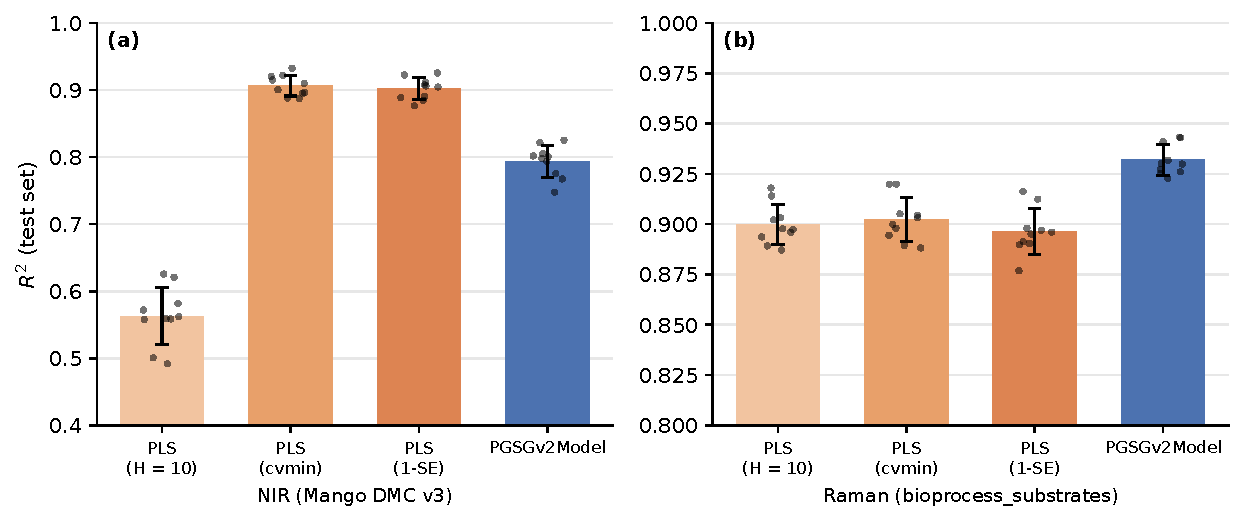
\includegraphics[width=0.7\linewidth]{h1_performance.pdf}
%DIFDELCMD < %%%
\DIFdelendFL \DIFaddbeginFL 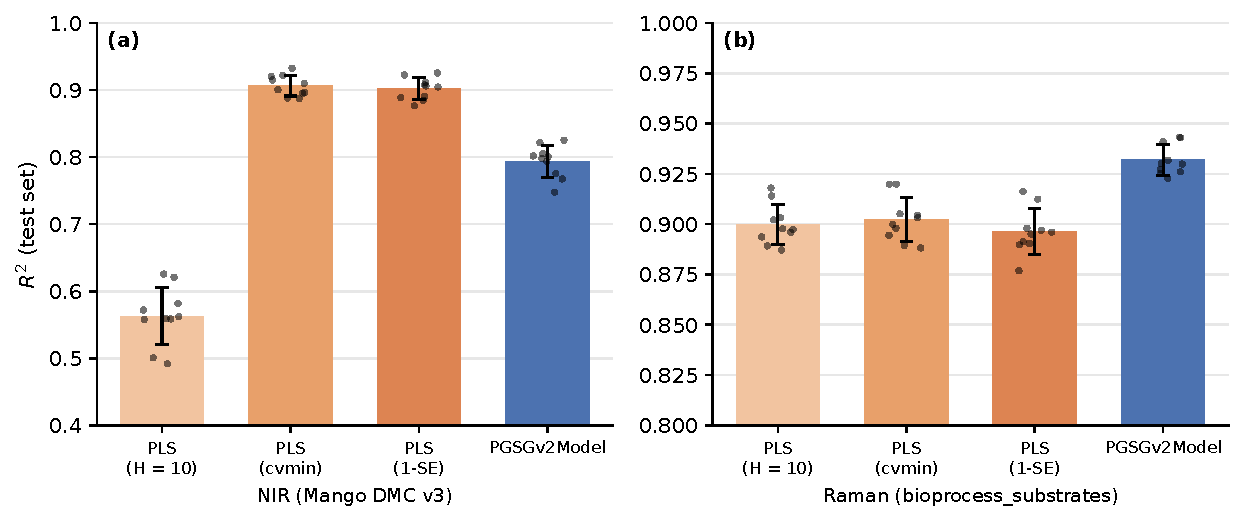
\includegraphics[width=\linewidth]{h1_performance.pdf}
\DIFaddendFL \caption{\DIFdelbeginFL \DIFdelFL{Predictive performance (}\DIFdelendFL \DIFaddbeginFL \DIFaddFL{H1: test-set }\DIFaddendFL $R^{2}$ \DIFaddbeginFL \DIFaddFL{over ten paired splits}\DIFaddendFL , \DIFdelbeginFL \DIFdelFL{held-out test set) of }\DIFdelendFL \DIFaddbeginFL \DIFaddFL{grouped by sample, for }\DIFaddendFL PLS \DIFaddbeginFL \DIFaddFL{with fixed $H=10$, PLS with cross-validated $H$ (cvmin }\DIFaddendFL and \DIFaddbeginFL \DIFaddFL{one-standard-error rules), and }\DIFaddendFL \texttt{PGSGv2Model}\DIFdelbeginFL \DIFdelFL{in each modality}\DIFdelendFL . \DIFaddbeginFL \DIFaddFL{Bars: mean; error bars: SD; points: individual splits.}\DIFaddendFL }
\label{fig:h1}
\end{figure}

\subsection{H2 and H3: gate topology across modalities}
\label{sec:results-h2h3}

\textbf{H2 (sparsity) is supported and robust to the functional form of the prior.} With each modality's original prior form, Hoyer sparsity is $S_{\mathrm{NIR}}=0.3176$ versus $S_{\mathrm{Raman}}=0.4150$ (Fig.~\ref{fig:h2h3}a). To rule out an encoding artifact --- the NIR prior is a step function, whereas the Raman prior is a Gaussian mixture --- the NIR prior was recoded as Gaussian bumps at the same literature centers and relative weights, matching the Raman encoding. The difference persists and widens ($S_{\mathrm{NIR}}=0.2345$ versus $S_{\mathrm{Raman}}=0.4150$), indicating that the effect is not attributable to prior-encoding style.

\textbf{H3 (smoothness) requires a methodological correction.} A first comparison of $\mathrm{TV}(g)$ by raw variable index yielded the result opposite to that predicted: $\mathrm{TV}_{\mathrm{NIR}}=0.0167 > \mathrm{TV}_{\mathrm{Raman}}=0.0076$ (Fig.~\ref{fig:h2h3}b). This reversal persisted under the Gaussian-prior ablation and is therefore not a prior-encoding artifact. Its cause is a difference in spectral sampling density: the NIR axis ($p=281$ variables over $\approx26{,}755$~cm$^{-1}$, $\approx95$~cm$^{-1}$ per variable) is approximately sixty times sparser, in wavenumber terms, than the Raman axis ($p=1{,}870$ variables over $\approx2{,}995$~cm$^{-1}$, $\approx1.6$~cm$^{-1}$ per variable). Total variation computed per variable index conflates the number of variables separating two informative regions with the smoothness of the transition per unit of physical spectrum, and is therefore an unsuitable metric for comparison across modalities with such disparate variable densities.

Recomputing smoothness per unit of physical bandwidth --- converting the NIR axis from nanometers to wavenumbers via $\tilde\nu=10^{7}/\lambda$ --- reverses the direction, now matching the hypothesis: $\mathrm{TV}_{\mathrm{physical,NIR}}=3.69\times10^{-4} \ll \mathrm{TV}_{\mathrm{physical,Raman}}=3.80\times10^{-3}$ (Fig.~\ref{fig:h2h3}c). This is corroborated by an independent check, unrelated to any gate or prior: the raw preprocessed spectrum is approximately $2.3$-fold rougher (point-to-point variation) in Raman than in NIR ($0.2156$ versus $0.0926$). Two independent measures agree once the density confound is removed. \textbf{H3 is supported}, provided smoothness is measured per unit of physical spectrum rather than per raw variable index; we note that the raw-index comparison is unreliable for cross-modality use in general and should be avoided in future work of this kind.

\begin{figure}[htbp]
\centering
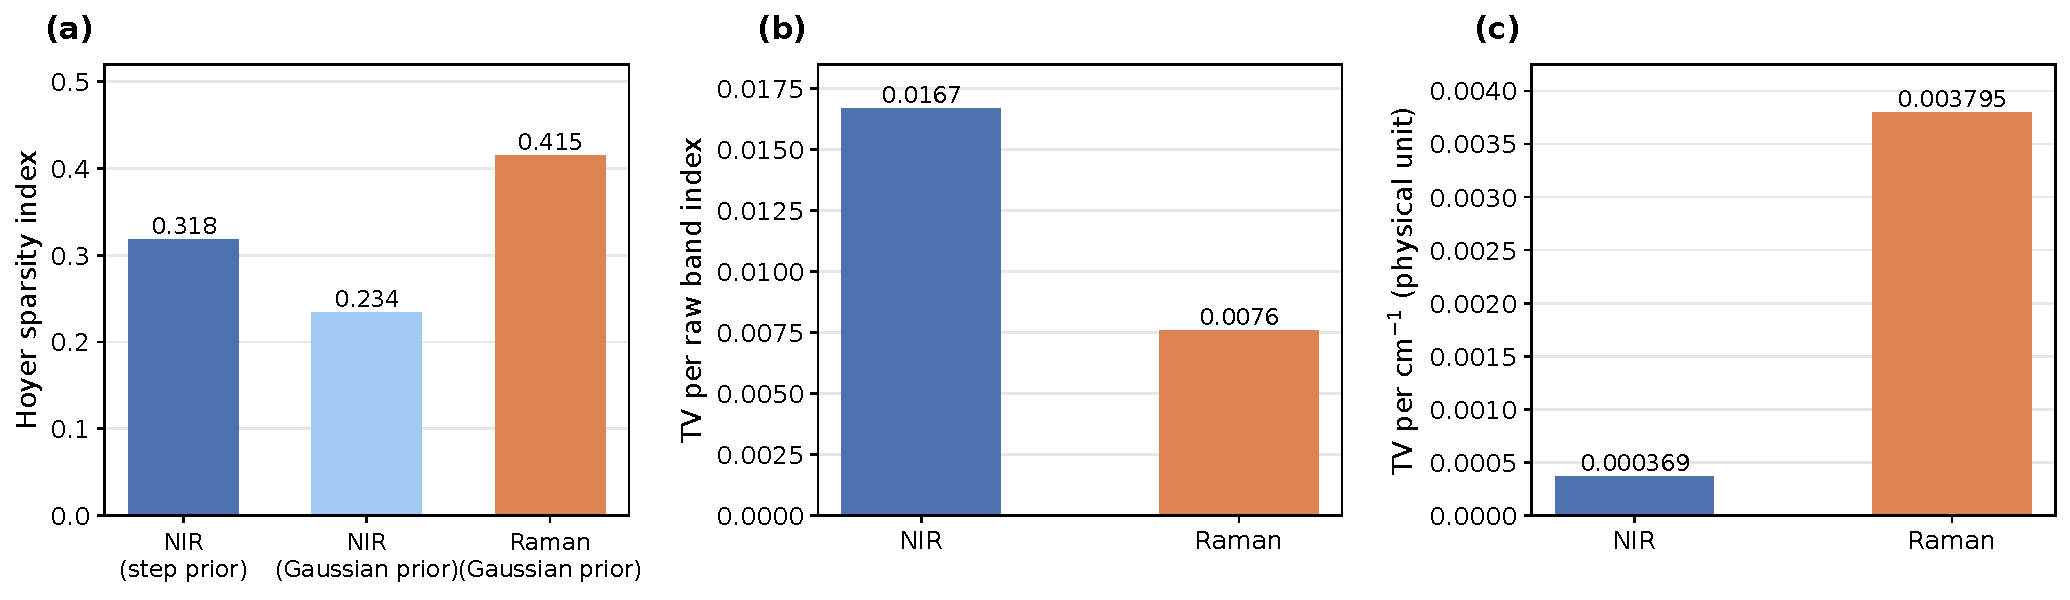
\includegraphics[width=\linewidth]{h2h3_topology.pdf}
\caption{Gate topology across modalities. (a) Hoyer sparsity: Raman more sparse than NIR under both prior encodings. (b) Smoothness by raw variable index: a misleading comparison, dominated by the difference in spectral sampling density between modalities. (c) Smoothness normalized by physical unit (cm$^{-1}$): the correct comparison, in agreement with raw-spectrum roughness.}
\label{fig:h2h3}
\end{figure}

\subsection{H4: value of a physically motivated prior}
\label{sec:results-h4}

Across ten training seeds per condition, predictive performance \DIFdelbegin \DIFdel{is statistically equivalent }\DIFdelend \DIFaddbegin \DIFadd{does not differ }\DIFaddend between literature-informed and uninformed (zero) initialization \DIFdelbegin \DIFdel{in both modalities }\DIFdelend \DIFaddbegin \DIFadd{beyond seed-to-seed variability in either modality }\DIFaddend (Table~\ref{tab:h4})\DIFaddbegin \DIFadd{; the differences in mean $R^{2}$ ($0.0050$ NIR, $0.0008$ Raman) are smaller than one standard deviation across seeds}\DIFaddend : NIR, $R^{2}_{\mathrm{lit}}=0.7933\pm0.0080$ versus $R^{2}_{\mathrm{rand}}=0.7983\pm0.0077$; Raman, $R^{2}_{\mathrm{lit}}=0.9302\pm0.0015$ versus $R^{2}_{\mathrm{rand}}=0.9310\pm0.0014$. Gate stability across seeds, in contrast, differs sharply and consistently in favor of the informed prior (Fig.~\ref{fig:h4}): pairwise gate correlation $\rho=0.9995$ (NIR, literature prior) versus $0.8653$ (NIR, uninformed), and $0.9976$ (Raman, literature prior) versus $0.8931$ (Raman, uninformed); pairwise Jaccard similarity of the top-weighted decile of variables, $0.9418$ (NIR, literature prior) versus $0.6002$ (NIR, uninformed), and $0.9011$ (Raman, literature prior) versus $0.6545$ (Raman, uninformed).

\begin{table}[htbp]
\centering
\caption{H4: performance and gate stability, literature prior versus uninformed initialization (10 seeds).}
\label{tab:h4}
\begin{tabular}{lcccc}
\toprule
& \multicolumn{2}{c}{NIR} & \multicolumn{2}{c}{Raman} \\
& Literature prior & Uninformed & Literature prior & Uninformed \\
\midrule
$R^{2}$ (mean $\pm$ SD) & $0.7933\pm0.0080$ & $0.7983\pm0.0077$ & $0.9302\pm0.0015$ & $0.9310\pm0.0014$ \\
$\rho$ (pairwise) & 0.9995 & 0.8653 & 0.9976 & 0.8931 \\
Jaccard (pairwise) & 0.9418 & 0.6002 & 0.9011 & 0.6545 \\
\bottomrule
\end{tabular}
\end{table}

\begin{figure}[htbp]
\centering
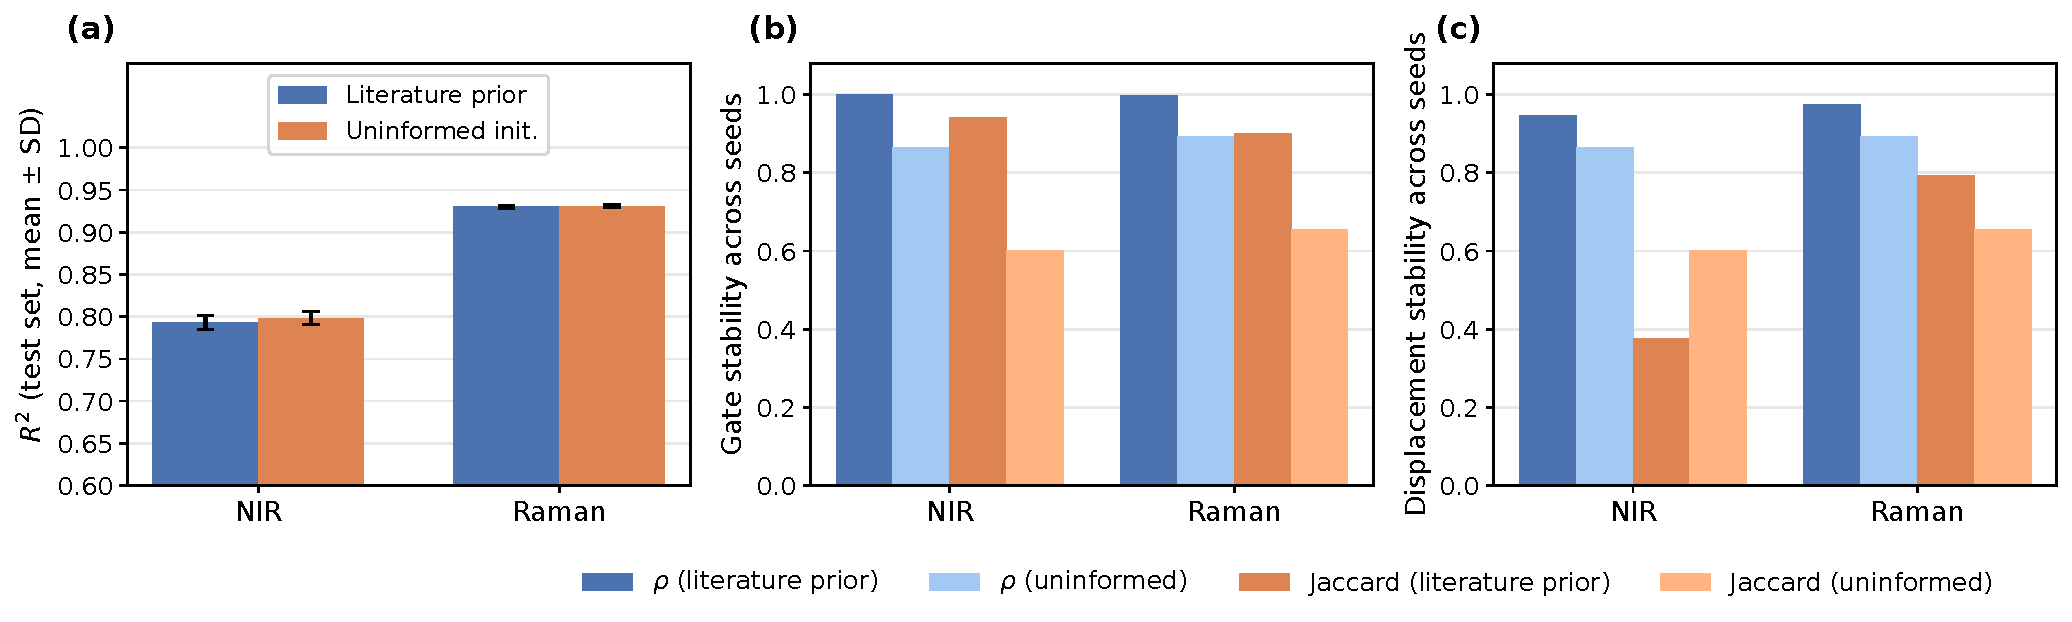
\includegraphics[width=\linewidth]{h4_prior_ablation.pdf}
\caption{H4: literature-informed prior versus uninformed initialization, 10 training seeds. (a) Predictive performance \DIFdelbeginFL \DIFdelFL{is statistically equivalent}\DIFdelendFL \DIFaddbeginFL \DIFaddFL{does not differ beyond seed-to-seed variability}\DIFaddendFL . (b) Gate stability across seeds is substantially higher with the literature-informed prior, in both modalities.}
\label{fig:h4}
\end{figure}

\textbf{H4 is supported for gate stability}; the accuracy component of the hypothesis (``equal to or better than'') \DIFdelbegin \DIFdel{holds only in the weak sense of statistical equivalence, not superiority, }\DIFdelend \DIFaddbegin \DIFadd{is not contradicted, but no superiority was observed, and equivalence was not formally tested (e.g., by two one-sided tests with a pre-declared margin), }\DIFaddend in either modality.

\subsection{H5: structure--physics correlation}
\label{sec:results-h5}

H5, as originally stated across modalities, is not testable as a statistical correlation with only two modalities ($n=2$). We reformulate it as a within-modality, band-by-band test in Raman, correlating literature-reported linewidths for twenty glucose Raman bands \cite{uspatent2024} against three descriptors extracted locally around each band from the trained gate, within an adaptive window capped at 45\% of the distance to the nearest neighboring literature band, to avoid cross-contamination between closely spaced bands such as the 1060/1073~cm$^{-1}$ pair. NIR is excluded from this quantitative test: it has only three literature bands, and its prior already encodes their exact literature widths by construction, which would render any correlation circular.

None of the three local descriptors yields a robust, correctly signed correlation (Fig.~\ref{fig:h5}, $n=20$): local gate full width at half maximum, $r=+0.254$ ($p=0.279$); local smoothness, $r=+0.048$ ($p=0.840$); local entropy, computed raw, $r=+0.407$ ($p=0.075$, marginal, correct direction), and normalized by window size ($\log n$), $r=-0.636$ ($p=0.003$, significant but in the direction opposite to that predicted). Diagnosis traced the entropy instability to the adaptive window itself: narrow windows, required near closely spaced bands, sample predominantly the flat top of a Gaussian bump, mechanically inflating normalized entropy toward its ceiling regardless of true local structure, whereas wider windows capture more of the true rise and fall, pulling the metric down. A synthetic control with a known, built-in correlation (gate bump width proportional to literature width by construction) confirmed that the extraction method recovers the expected correlation when it exists ($r=0.73$, $0.57$, and $-0.86$ for the three descriptors, all $p<0.01$), indicating that the null result on real data is informative rather than a failure of the extraction procedure. \textbf{H5 is not supported.} Further refinement of the windowing scheme was not pursued, to avoid the risk of adjusting a method until it yields the expected significance.

\begin{figure}[htbp]
\centering
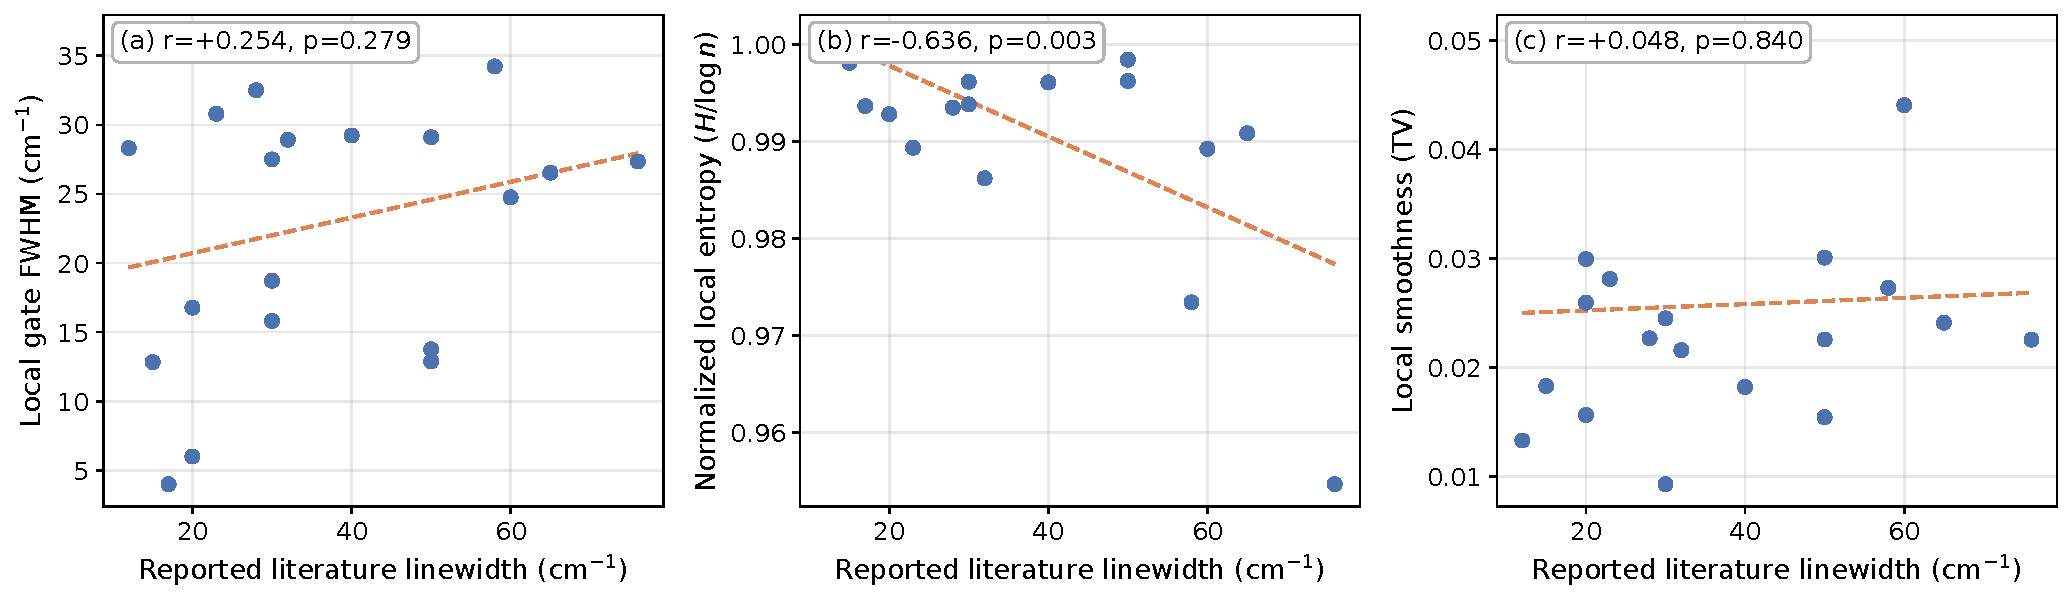
\includegraphics[width=\linewidth]{h5_correlation.pdf}
\caption{H5: literature-reported linewidth versus local gate descriptors, Raman, $n=20$ bands. Dashed lines show ordinary least-squares fits. None of the three descriptors shows a robust, correctly signed correlation.}
\label{fig:h5}
\end{figure}

\section{Discussion}
\label{sec:discussion}

Table~\ref{tab:summary} summarizes the outcome of the five hypotheses.

\DIFdelbegin %DIFDELCMD < \begin{table}[htbp]
%DIFDELCMD < \centering
%DIFDELCMD < \caption{Summary of hypothesis tests.}
%DIFDELCMD < \label{tab:summary}
%DIFDELCMD < \begin{tabular}{p{1cm}p{4.6cm}p{7.4cm}}
%DIFDELCMD < \toprule
%DIFDELCMD < Hyp. & Outcome & Key evidence \\
%DIFDELCMD < \midrule
%DIFDELCMD < H1 & Supported & $\Delta R^{2}_{\mathrm{PLS}}=+0.0246$ (Raman), $+0.2444$ (NIR); identical architecture \\
%DIFDELCMD < H2 & Supported, robust & Hoyer sparsity: Raman $0.415$ > NIR $0.235$--$0.318$ (two prior encodings) \\
%DIFDELCMD < H3 & Supported, with correction & Smoothness per cm$^{-1}$: NIR $3.69\times10^{-4} \ll$ Raman $3.80\times10^{-3}$; consistent with raw-spectrum roughness \\
%DIFDELCMD < H4 & Supported (stability); performance equivalent & Pairwise gate $\rho$: $0.998$--$0.9995$ (prior) versus $0.86$--$0.89$ (uninformed), both modalities \\
%DIFDELCMD < H5 & Not supported & No local descriptor correlates robustly with real per-band linewidth ($n=20$, Raman) \\
%DIFDELCMD < \bottomrule
%DIFDELCMD < \end{tabular}
%DIFDELCMD < \end{table}
%DIFDELCMD < %%%
\DIFdelend \DIFaddbegin \begin{table}[htbp]
\centering
\caption{Summary of hypothesis tests.}
\label{tab:summary}
\begin{tabular}{p{1cm}p{4.6cm}p{7.4cm}}
\toprule
Hyp. & Outcome & Key evidence \\
\midrule
H1 & Not supported (NIR); supported (Raman) & Paired $\Delta R^{2}$ vs.\ PLS-1se: $-0.108\pm0.031$ (NIR, 0/10 splits positive); $+0.036\pm0.007$ (Raman, 10/10) \\
H2 & Supported, robust & Hoyer sparsity: Raman $0.415$ > NIR $0.235$--$0.318$ (two prior encodings) \\
H3 & Supported, with correction & Smoothness per cm$^{-1}$: NIR $3.69\times10^{-4} \ll$ Raman $3.80\times10^{-3}$; consistent with raw-spectrum roughness \\
H4 & Supported (stability); no performance difference detected & Pairwise gate $\rho$: $0.998$--$0.9995$ (prior) versus $0.86$--$0.89$ (uninformed), both modalities \\
H5 & Not supported & No local descriptor correlates robustly with real per-band linewidth ($n=20$, Raman) \\
\bottomrule
\end{tabular}
\end{table}
\DIFaddend 

Taken together, the \DIFdelbegin \DIFdel{five results suggest a coherent mechanistic account. In both modalities the learned gate remains }\DIFdelend \DIFaddbegin \DIFadd{results separate two questions that the submitted version of this work had conflated: whether the gated model predicts better than PLS, and whether its gate carries interpretable, physically consistent structure. On the first question the answer depends on the modality, and in the direction opposite to the one originally reported. In NIR, a PLS model with some seventy latent variables captures the dry-matter signal of this heterogeneous, multi-cultivar season better than the shallow MLP; the large NIR advantage of the submitted version was an artifact of an under-parameterized baseline. In Raman, PLS saturates at four to eight latent variables and the gated MLP improves on it consistently. Because the learned gate stays }\DIFaddend close to its \DIFdelbegin \DIFdel{initializing prior }\DIFdelend \DIFaddbegin \DIFadd{initialization }\DIFaddend ($\rho\geq0.98$) \DIFaddbegin \DIFadd{and an uninformed initialization reaches the same accuracy (H4), this gain cannot be credited to the prior; it is more plausibly a property of the non-linear regressor, for instance its ability to represent interactions among the eight co-varying substrates of the bioprocess mixtures, which we did not test directly. The contrast between fixed-$H$ and calibrated comparisons is itself a methodological result: predictive claims for neural spectral models should be made only against a linear baseline whose complexity is selected by cross-validation, with training, validation, and test partitions that keep replicate spectra of a sample together. On the second question the answer is positive: gate topology differs between modalities in the direction predicted by their physics (H2}\DIFaddend , \DIFdelbegin \DIFdel{indicating that the model's advantage over PLS derives substantially from weighting the spectrum by chemically informed priorknowledge before regression rather than from extensive gradient-driven refinement of the gate. This reading also explains the difference in magnitude between the two modalities in H1: NIR spectra dilute analyte-relevant signal across many broad, overlapping, low-sparsity variables (H2, H3), so down-weighting uninformative regions substantially improves an otherwise weak PLS baseline ($R^{2}$ increasing from $0.568$ to $0.813$); Raman spectra are already sparse and narrow, so PLS applied to the raw spectrum already isolates the relevant signal ($R^{2}=0.904$), leaving comparatively little room for the prior weighting to add value ($R^{2}=0.929$)}\DIFdelend \DIFaddbegin \DIFadd{H3), provided the comparison is made per unit of physical spectrum}\DIFaddend .

H4 refines this picture further: the value of the prior lies not in predictive accuracy --- \DIFdelbegin \DIFdel{statistically indistinguishable}\DIFdelend \DIFaddbegin \DIFadd{indistinguishable, within seed-to-seed variability, }\DIFaddend with or without it --- but in the reproducibility of the learned attention pattern across independent training runs. A gate that points to different variables on every run is not a trustworthy explanation, even when its predictions are accurate; a physically motivated prior appears to function principally as an anchor for interpretability rather than as a performance lever.

H5, the single negative result, probes a stronger and more granular claim than H2/H3: not merely that aggregate gate topology differs between modalities in a manner consistent with physics (established by H2/H3), but that local gate structure, band by band, tracks the specific linewidth of each vibrational transition. With twenty Raman bands, none of the three descriptors tested produced a robust, replicable correlation, and the entropy descriptor proved unstable enough to reverse sign under a defensible alternative normalization. We interpret this as a resolution limit of the current descriptors rather than evidence that the gate is physically uninformative at a local level: gate topology appears to capture between-modality structural differences without necessarily resolving fine within-modality variation at the level of individual bands, at least with the windowing scheme used here.

\subsection{Limitations}

\DIFdelbegin \DIFdel{Three }\DIFdelend \DIFaddbegin \DIFadd{Five }\DIFaddend limitations apply across the study. First, the research process included \DIFdelbegin \DIFdel{a consequential correction}\DIFdelend \DIFaddbegin \DIFadd{two consequential corrections}\DIFaddend : an unpublished, superseded PGSG implementation was inadvertently used for an initial round of Raman experiments, \DIFdelbegin \DIFdel{producing a conclusion opposite to the one that holds under the correct architecture }\DIFdelend \DIFaddbegin \DIFadd{and the PLS baseline of the submitted version used a fixed number of latent variables; each reversed the conclusion for H1 in at least one modality at some stage }\DIFaddend (Section~\ref{sec:model-identity})\DIFdelbegin \DIFdel{; this is documented in full in }\DIFdelend \DIFaddbegin \DIFadd{, and both are documented in }\DIFaddend the public repository. Second, cross-modality topology comparisons require careful normalization by physical band density (Section~\ref{sec:results-h2h3}); future extensions of this line of work, including within the same research program, should adopt the same caution. Third, H4 was evaluated with ten training seeds per condition; a larger number would strengthen the stability estimate, although the observed effect is already large and consistent across both modalities. \DIFaddbegin \DIFadd{Fourth, the predictive comparison is restricted to PLS; comparisons with other attention-based architectures and with sparse linear models (Elastic Net, sparse PLS) were not performed and would be needed to position the model's accuracy more broadly. Fifth, only the H1 analysis uses sample-grouped splits: the gate analyses (H2--H5) use the original random reference split, in which replicate spectra of a sample can fall into both partitions, and the early-stopping validation subset of \texttt{PGSGv2Model} is selected by target value within the training partition, without regard to sample grouping. H4 compares two initializations on the same split, so its conclusion is unaffected, but its absolute $R^{2}$ values are slightly optimistic.
}\DIFaddend 

\section{Conclusion}

\DIFdelbegin \DIFdel{Prior-Guided Spectral Gating generalizes, }\DIFdelend \DIFaddbegin \DIFadd{Applied }\DIFaddend without architectural modification \DIFdelbegin \DIFdel{, from near-infrared to }\DIFdelend \DIFaddbegin \DIFadd{to NIR and }\DIFaddend Raman spectroscopy, \DIFdelbegin \DIFdel{and its learned gate }\DIFdelend \DIFaddbegin \DIFadd{Prior-Guided Spectral Gating outperforms a PLS baseline with cross-validated complexity in Raman but not in NIR, the reverse of the pattern obtained with a fixed number of PLS components; the NIR advantage reported in the submitted version of this work arose from an under-parameterized baseline. The learned gate nevertheless }\DIFaddend exhibits topological differences between the two modalities that are consistent with their \DIFdelbegin \DIFdel{underlying }\DIFdelend physical structure once compared on a physically meaningful basis\DIFdelbegin \DIFdel{. The magnitude of the predictive advantage, however, depends on how redundant or diluted the analyte-relevant signal already is in a given modality: substantial in NIR, modest in Raman. The principal contribution of a }\DIFdelend \DIFaddbegin \DIFadd{, and a }\DIFaddend literature-informed prior \DIFdelbegin \DIFdel{appears to be the reproducibility of the resulting interpretation }\DIFdelend \DIFaddbegin \DIFadd{makes the gate substantially more reproducible }\DIFaddend across training runs \DIFdelbegin \DIFdel{rather than raw }\DIFdelend \DIFaddbegin \DIFadd{without changing }\DIFaddend accuracy. A finer, band-level test of structure--physics correspondence did not succeed with the descriptors used here\DIFdelbegin \DIFdel{, a negative result reported alongside the positive ones. These findings inform }\DIFdelend \DIFaddbegin \DIFadd{. Because an uninformed initialization reaches the same accuracy, the Raman gain belongs to the non-linear regressor rather than to the prior. For }\DIFaddend subsequent stages of the \DIFdelbegin \DIFdel{broader }\DIFdelend research program (multi-target regression, \DIFdelbegin \DIFdel{systematic hyperparameter optimization, }\DIFdelend uncertainty quantification), \DIFdelbegin \DIFdel{for which the expected benefit of }\DIFdelend \DIFaddbegin \DIFadd{the case for }\DIFaddend spectral gating should \DIFdelbegin \DIFdel{be assessed on a case-by-case basis rather than assumed uniform across modalities and targets}\DIFdelend \DIFaddbegin \DIFadd{rest on the stability and physical interpretability of the gate, evaluated against calibrated linear baselines and with sample-grouped validation, rather than on an assumed predictive gain}\DIFaddend .

\section*{Data and code availability}
\label{sec:availability}
All code, experiment scripts, saved model outputs, and the commit history documenting the model-identity correction described in Section~\ref{sec:model-identity} are available at \url{https://github.com/clarimar/pgsg2-nir-raman-gating}. \DIFaddbegin \DIFadd{The repository includes a verified snapshot of the model and baseline implementations (\texttt{vendor/pgsg\_1}, with SHA-256 checksums), so that all experiments can be run from it alone. The Raman data were obtained through the \texttt{raman-data} package from the Hugging Face dataset \texttt{chlange/SubstrateMixRaman}, revision \texttt{887cf66d8cb25b2b953ee0a36889812f684de03e}.
}\DIFaddend 

\section*{Acknowledgments}
The authors gratefully acknowledge the Coordenação de Aperfeiçoamento de Pessoal de Nível Superior (CAPES), Brazil, for covering the Article Processing Charge (APC) of this publication under the CAPES--Elsevier Read and Publish Agreement (2026--2028)\DIFaddbegin \DIFadd{. This research did not receive any specific grant from funding agencies in the public, commercial, or not-for-profit sectors}\DIFaddend .

% *** PLACEHOLDER: to be completed with funding/acknowledgment information. ***

\bibliographystyle{elsarticle-num}
\bibliography{pgsg_2_refs}

\end{document}
 

 